\documentclass[iop,numberedappendix,apj,]{emulateapj}

\usepackage{epsfig}
\usepackage{amsmath}
\usepackage{rotating}
\usepackage{natbib}
\usepackage{enumerate}
\usepackage{multirow}
\usepackage{array}
\usepackage{appendix}
\usepackage{comment}
\usepackage{color,xcolor}
\usepackage{url}
\usepackage{hyperref}
\hypersetup{colorlinks,linkcolor={blue!50!black},citecolor={blue!50!black},urlcolor={blue!50!black}}
\allowdisplaybreaks[1]
\bibliographystyle{apj}
\renewcommand{\bibname}{References}

\def\plotonesc#1{\centering \leavevmode
\includegraphics[clip=, width=1.70\columnwidth]{#1}}
\def\plotoneh#1{\centering \leavevmode
\includegraphics[clip=, width=.95\columnwidth]{#1}}
\def\plotone#1{\centering \leavevmode
\includegraphics[clip=, width=.85\columnwidth]{#1}}
\def\plotoneShrinkSmall#1{\centering \leavevmode
\includegraphics[clip=, width=.49\columnwidth]{#1}}
\def\plotoneShrinkMed#1{\centering \leavevmode
\includegraphics[clip=, width=.55\columnwidth]{#1}}
\def\plotoneShrinkBig#1{\centering \leavevmode
\includegraphics[clip=, width=.65\columnwidth]{#1}}
\def\plottwo#1#2{\centering \leavevmode
\includegraphics[width=.45\columnwidth]{#1} \hfil
\includegraphics[width=.45\columnwidth]{#2}}
\def\plottwob#1#2{\centering \leavevmode
\includegraphics[width=.49\columnwidth]{#1} \hfil
\includegraphics[width=.49\columnwidth]{#2}}
\def\plottwor#1#2{\centering \leavevmode
\includegraphics[width=.55\columnwidth,angle=90]{#1} \hfil
\includegraphics[width=.55\columnwidth,angle=90]{#2}}
\def\plotthree#1#2#3{\centering \leavevmode
\includegraphics[width=.3\columnwidth]{#1} \hfil
\includegraphics[width=.3\columnwidth]{#2} \hfil
\includegraphics[width=.3\columnwidth]{#3}}

\def\gsim{\;\rlap{\lower 2.5pt
 \hbox{$\sim$}}\raise 1.5pt\hbox{$>$}\;}
\def\lsim{\;\rlap{\lower 2.5pt
   \hbox{$\sim$}}\raise 1.5pt\hbox{$<$}\;}

% set formatting properties
\setlength{\textwidth}{6.5in}
\setlength{\textheight}{8.8in}
\setlength{\hoffset}{0.0in}
\setlength{\voffset}{-0.4in}
\parindent 0.2in
\parskip 0.1in

\def\memoYF#1{\color{red}{\bf [#1]}\color{black}}

%%%%%%%%%%%%%%%%%%%%%%%%%%%%%%%%%%%%%%%%%%%%%%%%%
% THE DOCUMENT BEGINS HERE                      %
%%%%%%%%%%%%%%%%%%%%%%%%%%%%%%%%%%%%%%%%%%%%%%%%%

%\slugcomment{Submitted to ApJ, XX September 2015}

\begin{document}

\title{(tentative) Rotational Spectral Unmixing of Exoplanets}


\author{
%
Yuka Fujii\altaffilmark{1,2} 
%
Jacob Lustig-Yaeger\altaffilmark{3} 
%
Nicolas Cowan ?\altaffilmark{4} 
%
}

\affil{$^1$NASA Goddard Institute for Space Studies, 
  New York, NY 10025, USA}
      
\affil{$^2$Earth-Life Science Institute, Tokyo Institute of Technology, 
  Tokyo, 152-8550, JAPAN}
  
  
\affil{$^3$University of Washington, 
  }

\affil{$^4$McGill University, 
  }


\vspace{0.5\baselineskip}

\email{
yuka.fujii.ebihara@gmail.com
}

\begin{abstract}

\end{abstract}

\keywords{planets and satellites: Jupiter --- Sun: evolution ---
  planetary systems --- stars: evolution ---
  stars: AGB and post-AGB --- radio continuum: planetary systems}
  
%]%%% End front material



%%%%%%%%%%%%%%%%%%%%%%%%%%%%%%%%%%%%%%%%%%%%%%%%%%%%%%%%%%%%%%%%%%%
\section{Introduction}
\label{sec:intro}
%%%%%%%%%%%%%%%%%%%%%%%%%%%%%%%%%%%%%%%%%%%%%%%%%%%%%%%%%%%%%%%%%%%

Future direct imaging observations of terrestrial exoplanets is expected to play a vital role in characterizing Earth analogs in habitable zones and beyond. 
A substantial number of work have seeked detectable features in disk-integrated spectra of the Earth and other planets, as they are observed from an astronomical distance. 
It has been pointed out that not only some of atmospheric molecules are identifiable through spectral absorption features \citep[e.g.,][]{DesMarais2002} but also surface reflectance spectra affect the continuum of the spectra, which could be measured through low-resolution spectra, or multi-band photometry (color) \citep[e.g.,][]{Ford2001}. 

However, interpretation of disk-integrated colors is not trivial. 
This is particularly true for Earth-like planets which may harbor diverse atmospheric and surface characteristics including liquid water, partial cloud cover, continents, and possible biological surfaces, e.g. vegetation. 
Disentangling specific features from mixed disk-integrated color can be very challenging. 

A key here is to use time variation of the spectra; because the surface area that contributes to the scattered light changes due to planetary spin rotation and orbital revolution, the time variability can in principle be translated to the heterogeneity of the surface environment.  
\citet{Cowan2009, Cowan2011} performed Principal Component Analysis (PCA) on the observed multi-band photometry of the Earth, and found that number of surface types can be inferred from the number of dominant principle components (with a difference of 1) and that the variation pattern is indicative of the surface properties. 
\citet{Fujii2010, Fujii2011} decomposed multi-band photometric data of the Earth as a linear inverse problem, assuming the template reflectance spectra of the known major surface types, where they found that the relative abundance and the longitudinal variation of these surface types are reasonably recovered. 
Moreover, by coupling the time variation due to spin rotation and that due to orbital revolution, 2-dimensional information of the surface may be retrieved with sufficient quality of data \citep{Kawahara2010, Kawahara2011, Fujii2012}. 

\citet{Cowan2013} took another approach to the same inverse problem. 
Their strategy is to try to estimate the physically meaningful reflectance spectra and their distribution across the globe simultaneously, by making all of them fitting parameters and letting them to fit the data. 
The result appeared successful to the extent that the obtained reflectance spectra roughly match the typical spectra of clouds, ocean, and continents. 
However, the longitudinal map of these components do not match the reality sufficiently well. 

We were motivated by this unsatisfactory result and decided to revisit their analysis with some updates. 
Specifically, the updates include:
\begin{itemize}
\item Revisiting the formulation and point out the inherit degeneracy. 
\item Introducing regularization terms
\item Influence of the unknown radius
\end{itemize}

The organization of this paper is as follows. 
Section \ref{s:frame} revisits the problem, ...

%%%%%%%%%%%%%%%%%%%%%%%%%%%%%%%%%%%%%%%%%%%%%%%%%%%%%%%%%%%%%%%%%%%
\section{Framing the problem}
\label{s:frame}
%%%%%%%%%%%%%%%%%%%%%%%%%%%%%%%%%%%%%%%%%%%%%%%%%%%%%%%%%%%%%%%%%%%


%%%%%%%%%%%%%%%%%%%%%%%%%%%%%%%%%%%%%%%%%%%%%%%%%%%%%%%%%%%%%%
\subsection{Algebraic Formulation}
\label{ss:model}
%%%%%%%%%%%%%%%%%%%%%%%%%%%%%%%%%%%%%%%%%%%%%%%%%%%%%%%%%%%%%%

Assuming that the planetary surface is Lambertian scatterer everywhere, with a certain number $K$ of mutually distinct surface types, 
the disk-integrated spectra can be written as a weighted summation of the reflectance spectra of different surface types, e.g., 
%%%
\begin{equation}
d_{ij} = R_p^2 \sum _{i,k} f_{ik}^{\ast } \, s_{kj}
\end{equation}
%%%
where $R_p$ is the planetary radius, $i$, $j$, and $k$ are indices for the observation epochs, bands, and the surface types, respectively \citep[see][]{Fujii2010} . 
The symbols represent as follows:
$d_{ij}$ is the observed apparent albedo (``$d$'' for data) at $i$-th epoch and $j$-th band, 
$f_{lk}^{\ast }$ is the contribution factor of the $k$-th surface type at $i$-th observational epoch, and 
$s_{kj}$ is the reflectance spectra of $k$-th surface type at $j$-th band. 
The maximum number of $i$, $j$ and $k$ will be denoted by $I$, $J$, and $K$, below, as summarized in Table \ref{tab:index}. 

%%%%%%%%%%%%%%%%%%%%%%%%%%%%%%%%%%%
\begin{table}[bh]
\caption{Indexes}
\begin{center}
\begin{tabular}{ccc} \hline \hline
Name & Symbol & Maximum \\ \hline
Observation Time & $i$ & I \\
Band & $j$ & J  \\
Surface Type & $k$ & K  \\
Longitudinal Slice  & $l$ & L \\ \hline
\end{tabular}
\end{center}
\label{tab:index}
\end{table}%
%%%%%%%%%%%%%%%%%%%%%%%%%%%%%%%%%%%


The contribution factor $f^{\ast }$ is the weighted summation of the area fraction of $k$-th surface type, i. e.,
%%%
\begin{equation}
f^{\ast }_{ik} = \sum _{l} W_{il} f_{lk}
\end{equation}
%%%
where $l$ is the index for longitudinal slices, $f_{lk}$ is the area fraction of the $k$-th surface type at $l$-th longitudinal slice, and 
$W_{il}$ is the weight function for $i$-th epoch and $l$-th longitudinal slice which depends only on the observational geometry. 
The maximum number of $l$ is denoted by $L$. 
As a result,
%%%
\begin{equation}
d_{ij} = R_p^2 \sum _{l,k} W_{il} \, f_{lk} \, s_{kj}
\end{equation}
%%%

Because $f$ is area fraction and $s$ is reflectance spectra, they are subject to the following constraints:
%%%
\begin{eqnarray}
\begin{cases}
\;\; 0 < s_{kj} < 1 \;\;\; & \mbox{for any $k$, $j$} \\
\;\; 0 < f_{lk} < 1 \;\;\; & \mbox{for any $l$, $k$} \\
\;\; \sum_k f_{lk} = 1 & \mbox{for any $l$} 
\end{cases}
\label{eq:constraints}
\end{eqnarray}
%%%

Now, in the case that the planetary radius and observational geometry (latitude and longitude of the sub-stellar point and the sub-observer point) is fully known, the relevant problem is, given $d_{ij}$, estimate both $f_{lk}$ and $s_{kj}$ subject to the constraints of equation (\ref{eq:constraints}). 
---This is pioneered by trial by \citet{Cowan2013}. 

We argue that estimating $f$ and $s$ is no superior to estimating $f^*$ and $s$ subject to the following similar constraint:
%%%
\begin{eqnarray}
\begin{cases}
\;\; 0 < s_{kj} < 1 \;\;\; & \mbox{for any $k$, $j$} \\
\;\; 0 < f^{\ast }_{lk} < 1 \;\;\; & \mbox{for any $l$, $k$} \\
\;\; \sum_k f_{lk}^{\ast } = 1 & \mbox{for any $l$} 
\end{cases}
\label{eq:constraints_ast}
\end{eqnarray}
%%%
\memoYF{write here}.

%%%%%%%%%%%%%%%%%%%%%%%%%%%%%%%%%%%%%%%%%%%%%%%%%%%%%%%%%%%%%%
\subsection{Degeneracy}
\label{ss:degeneracy}
%%%%%%%%%%%%%%%%%%%%%%%%%%%%%%%%%%%%%%%%%%%%%%%%%%%%%%%%%%%%%%


%%%
\begin{equation}
\tilde d_{ij} = \sum _{i,k} f_{ik}^{\ast } \, s_{kj}
\end{equation}
%%%
where $\tilde d_{ij} = d_{ij}/R_p^2$. 
Without any constraints on $f^{\ast }$ and $s$, it is trivial to notice the degeneracy in the solutions. 
Using an arbitrary regular matrix $X$ with rank $K$, a particular set of solution $\{ f^{\ast },\,s\}$ implies another set of solution $\{ f^{\ast }X^{-1},\,Xs\}$. 

Now that they are subject to the constraints (equation (\ref{eq:constraints_ast})), the range of acceptable solution is limited. 
However, the constraints cannot be sufficient to reduce them to a unique solution. 
One can create a infinite number of candidates for $f_{ik}^{\ast }$ which satisfies both of the two constraints for $f$, then $s$ may be obtained by $s = f^{+} \tilde d$, where $f^+$ is the pseudo-inverse matrix (note that $K < I$ to be able to find the solution) and among these solutions there should be many that satisfy the constraint for $s$ as well. 
\memoYF{Need to brush up. Possibly need to consider SVD of $f$. }

To see this, we demonstrate the application to the mock data with known solution in Section \ref{s:mockdata}.

%%%%%%%%%%%%%%%%%%%%%%%%%%%%%%%%%%%%%%%%%%%%%%%%%%%%%%%%%%%%%%
\subsection{Bayesian Formulation}
\label{ss:regularization}
%%%%%%%%%%%%%%%%%%%%%%%%%%%%%%%%%%%%%%%%%%%%%%%%%%%%%%%%%%%%%%

%%%
\begin{eqnarray}
Posterior = \prod\limits_{i,j} \frac{1}{\sqrt{2\pi }\sigma_{ij}} &&  \exp \left[ - \frac{(d_{ij} - \sum _{lk} W_{il} f_{lk} s_{kj})^2}{2 \sigma _{ij}^2} \right] \notag \\
&& \times \; \mathcal{P} (\{f_{l,k}\}) \cdot \mathcal{P}(\{s_{l,k}\}) 
\end{eqnarray}
%%%
where $\mathcal{P} (X) $ is a prior for $X$. 

In order to take account of constraints (equation (\ref{eq:constraints})), we adopt the following transformation of variables: 
%%%
\begin{eqnarray}
\begin{cases}
t_{kj} = \displaystyle \ln \left[ \frac{ s_{kj} }{1 - s_{kj} } \right]  \;\;\; & \mbox{for any $k$, $j$} \\
g_{lk} = \displaystyle \ln \left[ \frac{ f_{lk} }{1 - \sum _{m=0}^{k} f_{lm} } \right] \;\;\; & \mbox{for $k=1, ..., K-1$, any $j$} 
\end{cases}
\end{eqnarray}
%%%
Note that there is a 1-to-1 correspondence between $t$ and $s$ or $g$ and $f$ where $s$ and $f$ always satisfy our constraints. 

\newpage

%%%%%%%%%%%%%%%%%%%%%%%%%%%%%%%%%%%%%%%%%%%%%%%%%%%%%%%%%%%%%%%%%%%
\section{Test with idealized mock data}
\label{s:mockdata}
%%%%%%%%%%%%%%%%%%%%%%%%%%%%%%%%%%%%%%%%%%%%%%%%%%%%%%%%%%%%%%%%%%%

%%%%%%%%%%%%%%%%%%%%%%%%%%%%%%%%%%%%%%%%%%%%%%%%%%%%%%%%%%%%%%
\subsection{Creating Mock Data}
\label{ss:createmockdata}
%%%%%%%%%%%%%%%%%%%%%%%%%%%%%%%%%%%%%%%%%%%%%%%%%%%%%%%%%%%%%%


Before applying to the observed data, we shall demonstrate the analysis procedure with a mock dataset with the known answer. 
For this purpose, we use a simplified albedo map of the Earth based on the IGBP classification. 
We re-classify the IGBP map into four surface types, ``ocean', ``vegetation', and ``soil'' and following Table 2 of \citet{Fujii2010} except that we merge ``snow'' into ``soil'' considering its small fraction. 
The upper left panel of Figure \ref{fig:mockdata} depicts such an surface classification. 
The reflectance spectra for these three surface types ($s_{kj}$) are adopted from ASTER spectral library \citep{Baldridge2009} in the same way as \citet{Fujii2010} (Figure 7 in that paper), and are shown in the upper right panel of Figure \ref{fig:mockdata}. 

We then compute the geometrically weighted area fraction of each surface type (``contribution factor'' or $f^{\ast }_{ik}$) assuming an equatorial view at the quadrature \memoYF{Describe in more detail.}; this is shown in the lower left panel of Figure \ref{fig:mockdata}. 
Using $s_{kj}$ and $f^{\ast }_{ik}$, we compute the apparent albedo at each observation frame, on the assumption that the surfaces are ``Lambert'' scatterers. The effect of atmosphere is completely ignored. 
The mock lightcurves created through the above-mentioned procedure is presented in the lower right panel of Figure \ref{fig:mockdata}. 

%%%%%%%%%%%%%%%%%%%%%%%%%%%%%%%%%%%
\begin{figure*}[!bpth]
    \begin{minipage}{0.5\hsize}
    \begin{center}
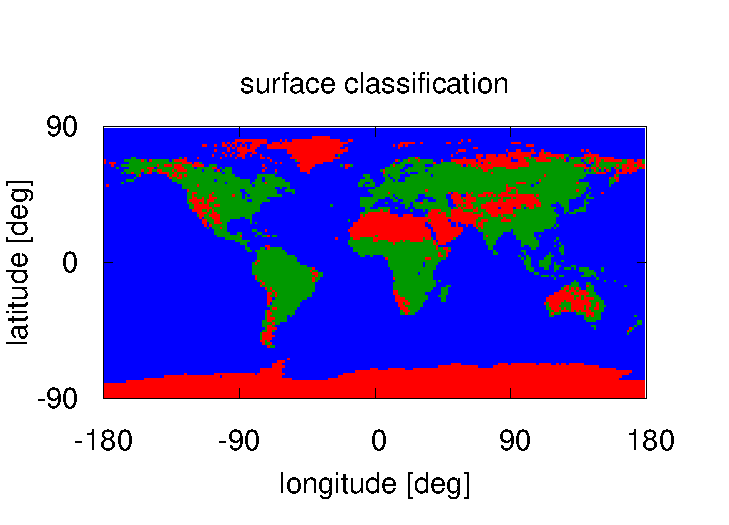
\includegraphics[width=\hsize]{IGBP_simplemap.pdf}
    \end{center}
     \end{minipage}
  \begin{minipage}{0.5\hsize}
    \begin{center}
    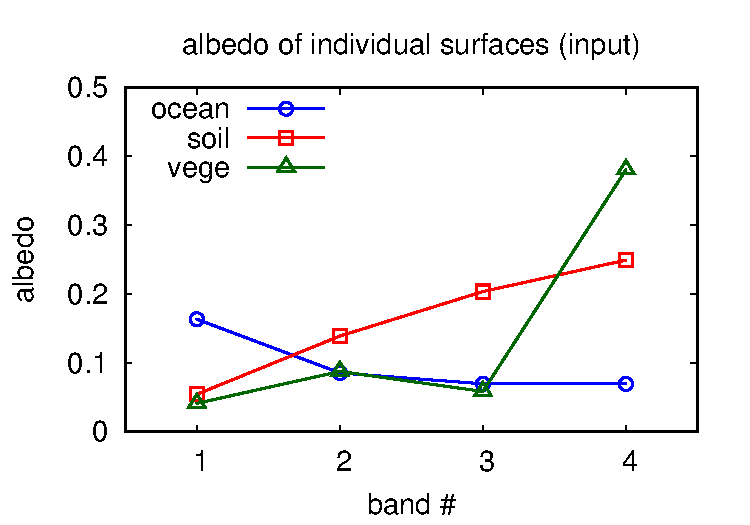
\includegraphics[width=\hsize]{mockdata_quadrature_bandsp.pdf}
    \end{center}
\end{minipage}
  \begin{minipage}{0.5\hsize}
    \begin{center}
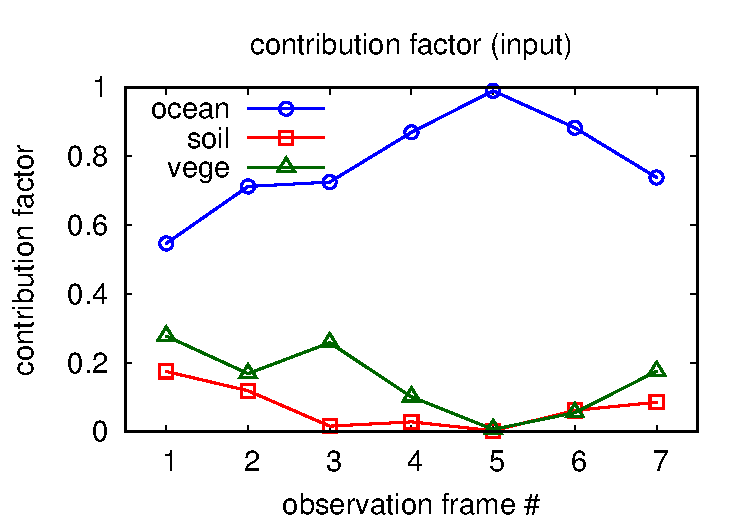
\includegraphics[width=\hsize]{mockdata_quadrature_factor.pdf}
    \end{center}
 \end{minipage}
   \begin{minipage}{0.5\hsize}
    \begin{center}
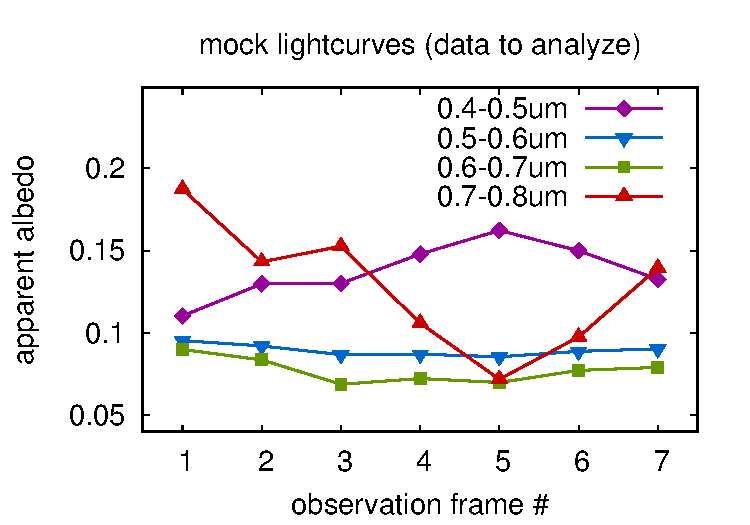
\includegraphics[width=\hsize]{mockdata_quadrature_lc.pdf}
    \end{center}
 \end{minipage}
    \caption{Our mock data based on Earth surface. }
\label{fig:mockdata}
\end{figure*}
%%%%%%%%%%%%%%%%%%%%%%%%%%%%%%%%%%%





\newpage


%%%%%%%%%%%%%%%%%%%%%%%%%%%%%%%%%%%%%%%%%%%%%%%%%%%%%%%%%%%%%%
\subsection{Testing Rotational Unmixing with Mock Data}
\label{ss:testmockdata}
%%%%%%%%%%%%%%%%%%%%%%%%%%%%%%%%%%%%%%%%%%%%%%%%%%%%%%%%%%%%%%


\newpage

%%%%%%%%%%%%%%%%%%%%%%%%%%%%%%%%%%%%%%%%%%%%%%%%%%%%%%%%%%%%%%%%%%%
\section{Application to 4 EPOXI observations of the Earth}
\label{s:epoxi}
%%%%%%%%%%%%%%%%%%%%%%%%%%%%%%%%%%%%%%%%%%%%%%%%%%%%%%%%%%%%%%%%%%%

%%%%%%%%%%%%%%%%%%%%%%%%%%%%%%%%%%%%%%%%%%%%%%%%%%%%%%%%%%%%%%
\subsection{EPOXI data}
\label{ss:epoxidata}
%%%%%%%%%%%%%%%%%%%%%%%%%%%%%%%%%%%%%%%%%%%%%%%%%%%%%%%%%%%%%%

%%%%%%%%%%%%%%%%%%%%%%%%%%%%%%%%%%%
\begin{figure*}[!tb]
    \begin{center}
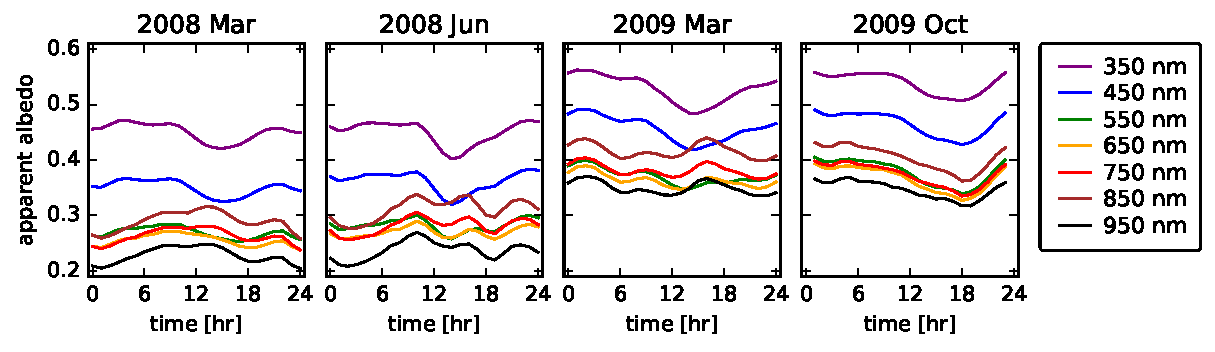
\includegraphics[width=\hsize]{EPOXI_vislightcurve_4obs.pdf}
    \end{center}
    \caption{4 light curves of the Earth obtained with EPOXI mission.}
\label{fig:EPOXIlc}
\end{figure*}
%%%%%%%%%%%%%%%%%%%%%%%%%%%%%%%%%%%

We now apply our framework to the observed multi-band reflected light curves of the Earth obtained with EPOXI \citep{Livengood2011, Cowan2011}. 
There are 7 photometric filters from about 300 nm to 1000 nm, each of which has roughly 100-nm band width. 
In total, 5 series of observations were conducted, each of which spans $\sim $24 hours with 1-hour intervals. 
Since one of them includes lunar transit in front of the Earth and the interpretation is not straightforward, we just remove it from our data and consider only 4 series of observations, which were conducted on March 2008, June 2008, March 2009, and October 2009. 
The data are presented in Figure \ref{fig:EPOXIlc} in terms of {\it apparent albedo}, the planetary intensity normalized by that of a loss-less Lambert sphere with the same radius and at the same phase \citep{Qiu2003, Seager2010}. 

The geometrical configuration among the star, the target (the Earth), and the detector varies from observation to observation. 
The information is summarized in \citet{Cowan2011}, but we also outline in Table \ref{tab:EPOXI} just for reference. 

%%%%%%%%%%%%%%%%%%%%%%%%%%%%%%%%%%%
\begin{figure*}[!bt]
    \begin{center}
    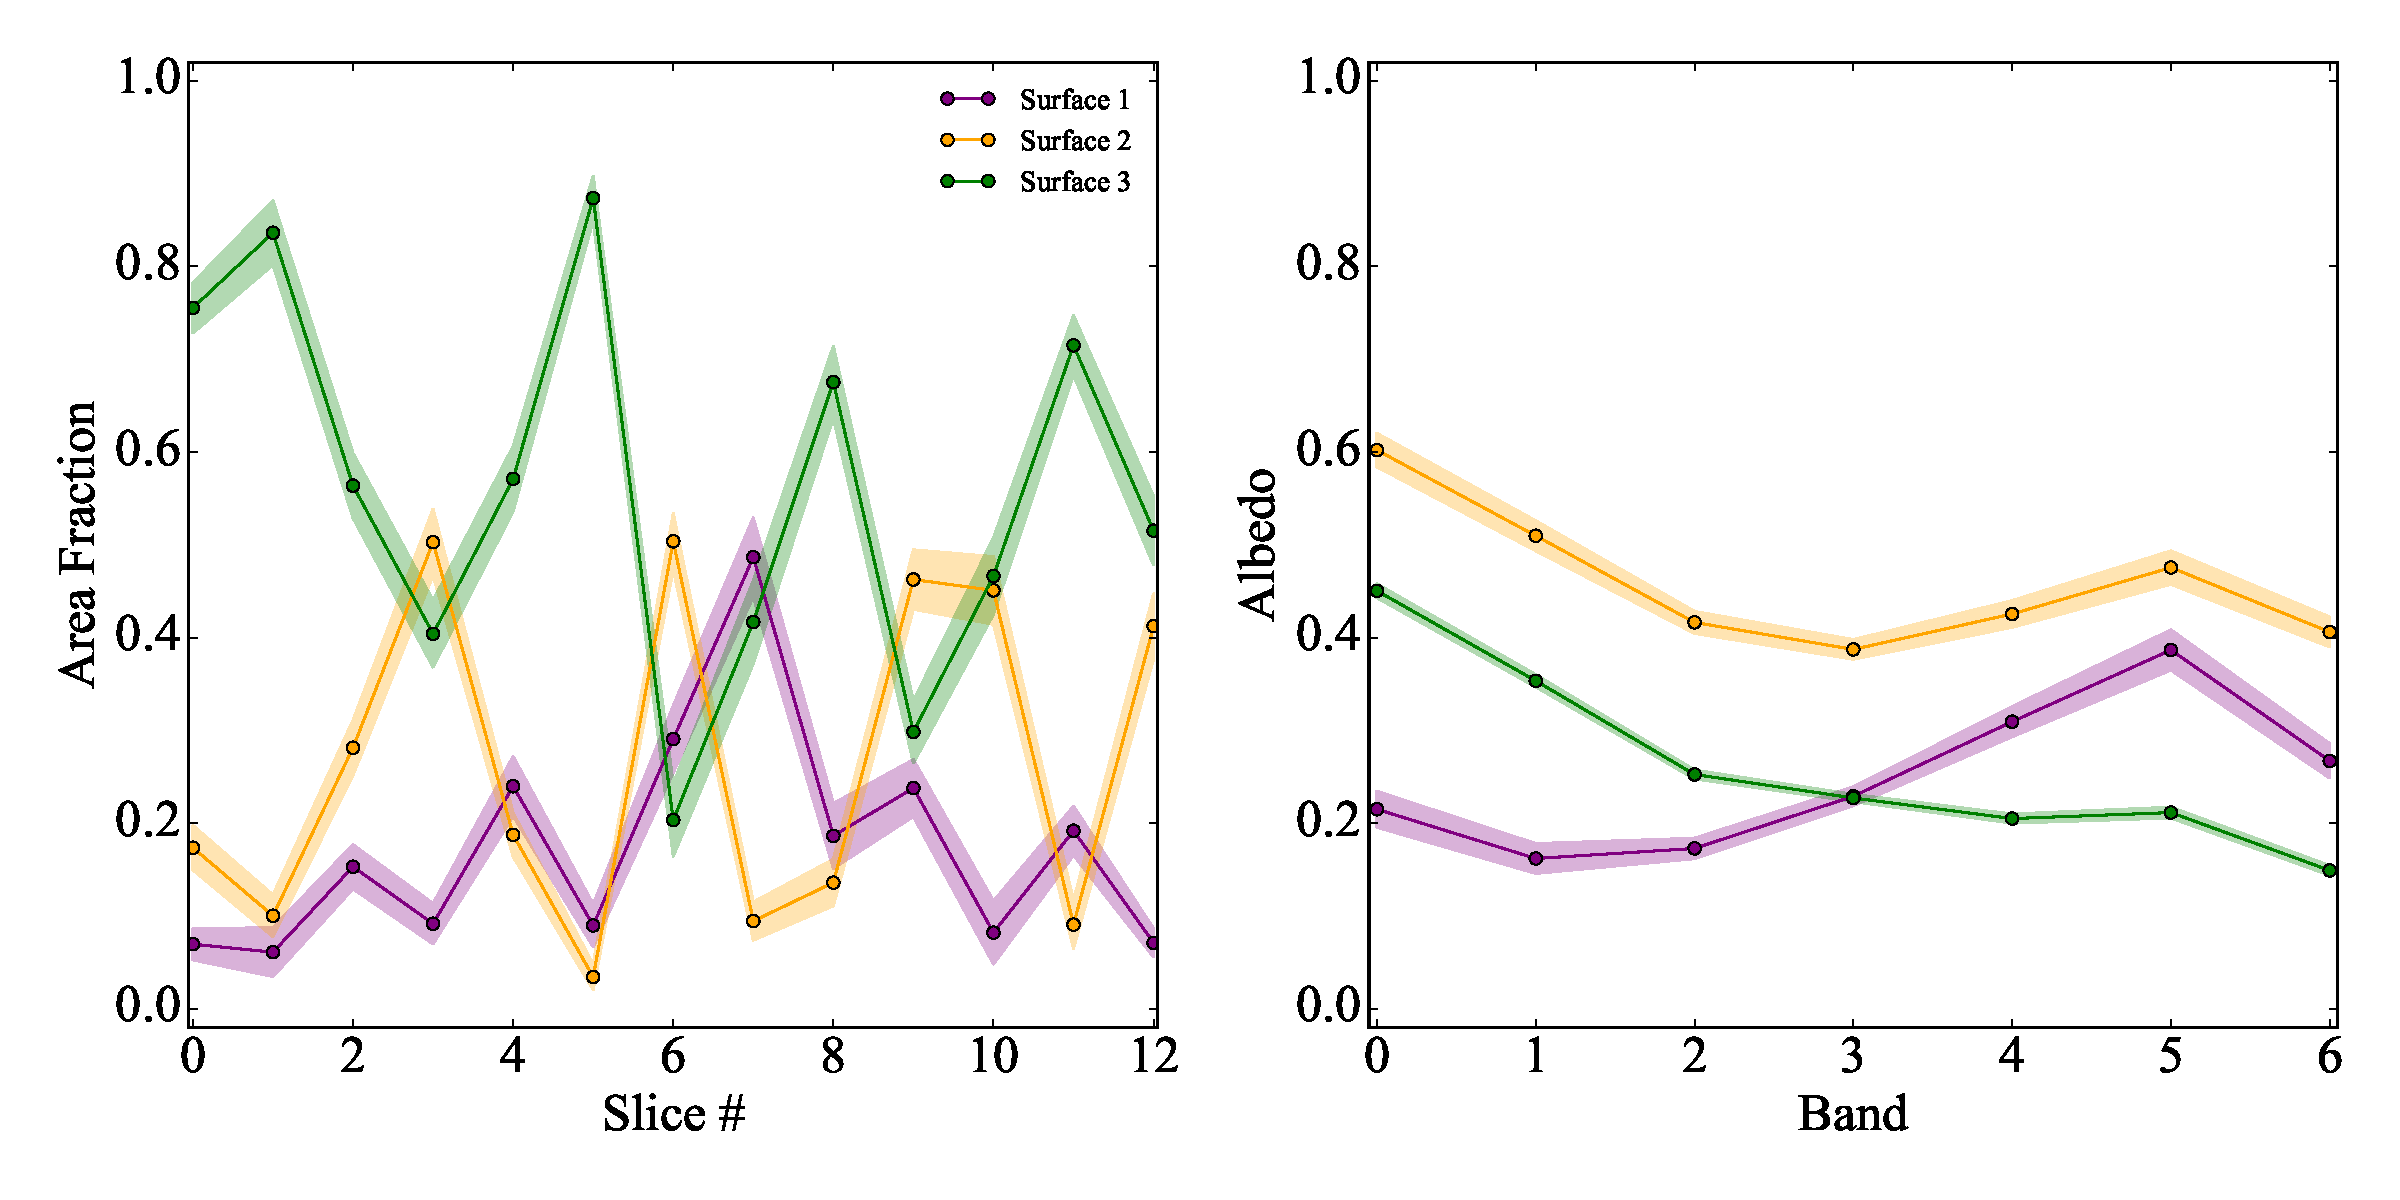
\includegraphics[width=\hsize]{June_xmed_std_GPReg.pdf}
    \end{center}
    \caption{Result of inversion of EPOXI June data. \memoYF{to be revised}}
\label{fig:mcmc_June_tmp}
\end{figure*}
%%%%%%%%%%%%%%%%%%%%%%%%%%%%%%%%%%%

%%%%%%%%%%%%%%%%%%%%%%%%%%%%%%%%%%%
\begin{table*}[htp]
\caption{EPOXI Observations}
\begin{center}
\begin{tabular}{lcccc} \hline \hline
& Equator (equinox) & Equator (solstice) & North & South \\ \hline
Date & 2008 Mar 18-19 & 2008 Jun 4-5 & 2009 Mar 27-28 & 2009 Oct 4-5 \\ 
Phase & $57.7^{\circ }$ & $76.6^{\circ }$ & $85.9^{\circ }$ & $86.4^{\circ }$ \\ 
average sub-solar latitude & $-0.4^{\circ }$ & $22.6^{\circ }$ & $3.0^{\circ }$ & $-4.6^{\circ }$ \\
average sub-observer latitude & $1.6^{\circ }$ & $0.3^{\circ }$ & $61.5^{\circ }$ & $-73.7^{\circ }$  \\
initial sub-solar longitude & $267.6^{\circ }$ & $286.0^{\circ }$ & $296.7^{\circ }$ & $33.2^{\circ }$ \\
initial sub-observer longitude & $210.1^{\circ }$ & $210.5^{\circ }$ & $210.1^{\circ }$ & $300.6^{\circ }$ \\ \hline
\end{tabular}
\end{center}
\label{tab:EPOXI}
\end{table*}%
%%%%%%%%%%%%%%%%%%%%%%%%%%%%%%%%%%%

%%%%%%%%%%%%%%%%%%%%%%%%%%%%%%%%%%%%%%%%%%%%%%%%%%%%%%%%%%%%%%
\subsection{Retrieval using equation (\ref{eq:}) }
\label{ss:retrieval}
%%%%%%%%%%%%%%%%%%%%%%%%%%%%%%%%%%%%%%%%%%%%%%%%%%%%%%%%%%%%%%

First, each series of data is analyzed separately. 
Without regularization and with regularization

%%%%%%%%%%%%%%%%%%%%%%%%%%%%%%%%%%%%%%%%%%%%%%%%%%%%%%%%%%%%%%%%%%%
\section{Discussion}
\label{s:discussion}
%%%%%%%%%%%%%%%%%%%%%%%%%%%%%%%%%%%%%%%%%%%%%%%%%%%%%%%%%%%%%%%%%%%


%%%%%%%%%%%%%%%%%%%%%%%%%%%%%%%%%%%%%%%%%%%%%%%%%%%%%%%%%%%%%%
\subsection{Uncertainty in Radius}
\label{ss:radius}
%%%%%%%%%%%%%%%%%%%%%%%%%%%%%%%%%%%%%%%%%%%%%%%%%%%%%%%%%%%%%%

%%%%%%%%%%%%%%%%%%%%%%%%%%%%%%%%%%%%%%%%%%%%%%%%%%%%%%%%%%%%%%
\subsection{Sensitivity to Initial Condition}
\label{ss:initialcondition}
%%%%%%%%%%%%%%%%%%%%%%%%%%%%%%%%%%%%%%%%%%%%%%%%%%%%%%%%%%%%%%


%%%%%%%%%%%%%%%%%%%%%%%%%%%%%%%%%%%%%%%%%%%%%%%%%%%%%%%%%%%%%%%%%%%
\section{Summary}
\label{s:summary}
%%%%%%%%%%%%%%%%%%%%%%%%%%%%%%%%%%%%%%%%%%%%%%%%%%%%%%%%%%%%%%%%%%%




\acknowledgments

\bibliography{ref}



\end{document}
